% MODEL CALIBRATION
We now turn towards model calibration.
The goal is to infer the unknown hydrological parameters with the available outflow data.
Two different Bayesian models are employed in order to account for the high level of uncertainty and error in hydrological model predictions \cite{Hydro:DelGiudice2013,Hydro:DelGiudice2015}.
According to the first simple model, the hydrological parameters and the measurement uncertainty are unknown.
The formulation is the nonlinear generalization of the inverse modeling with an unknown noise level that was discussed in \cref{sec:Bayesian:InverseProblems:LinearRegression}.
In addition to that, a second model is devised that considers also error correlation and model discrepancy as a function of time.
The main behavior of the outflow is captured by the model, while a simple trend function accounts for the discrepancy.
This more advanced representation of simulator discrepancy was already highlighted in \cref{sec:Bayesian:InverseProblems:ModelUncertainties}.
\par % MEASUREMENT DATA
The measurement data \(\bm{y} = (y_0,\ldots,y_{600})^\top\) comprise the observations of the outflow \(y_i = Q(t_i)\) for \(i=0,\ldots,600\).
They are represented as responses \(\tilde{\bm{y}} = \mathcal{M}_{\bm{d}}(\bm{x})\) of the forward model in \cref{eq:Hydro:ForwardModel}
contaminated by random measurement noise and systematic model discrepancy.
The unknown parameters of the forward and the error model can then be identified in a statistical data analysis.

\subsection{Independent random errors}
% DATA MODEL
A first simple model takes only random measurement errors into account.
They are assumed to act additively and independently on the forward model predictions.
Thus the measured data are represented as
\begin{equation} \label{eq:Hydro:Simple:NoisyData}
  \bm{y} = \mathcal{M}_{\bm{d}}(\bm{x}) + \bm{\varepsilon}.
\end{equation}
Here, \(\bm{\varepsilon}\) is a realization of a random vector with a Gaussian distribution
\(\pi(\bm{\varepsilon} \cond \sigma) = \mathcal{N}(\bm{\varepsilon} \cond \bm{0},\sigma^2 \bm{I})\), where the noise level \(\sigma > 0\) is unknown.
Consequently the following statistical model arises
\begin{equation} \label{eq:Hydro:Simple:RandomData}
  \pi_1(\bm{y} \cond \bm{x},\sigma) = \mathcal{N}(\bm{y} \cond \mathcal{M}_{\bm{d}}(\bm{x}), \sigma^2 \bm{I}).
\end{equation}
% POSTERIOR DISTRIBUTION
The likelihood function is simply \(\mathcal{L}_1(\bm{x},\sigma) = \mathcal{N}(\bm{y} \cond \mathcal{M}_{\bm{d}}(\bm{x}), \sigma^2 \bm{I})\).
Instead of merely maximizing the likelihood, a fully Bayesian approach is pursued.
For any given prior distribution \(\pi_1(\bm{x},\sigma)\), the corresponding posterior is
\begin{equation} \label{eq:Hydro:Simple:Posterior}
  \pi_1(\bm{x},\sigma \cond \bm{y}) \propto \mathcal{L}_1(\bm{x},\sigma) \pi_1(\bm{x},\sigma).
\end{equation}
\par % PRIOR DISTRIBUTIONS
In order to complete the setup, we specify a joint prior of the unknowns with the product structure
\(\pi_1(\bm{x},\sigma) = \pi_1(\bm{x}) \pi_1(\sigma)\) and \(\pi_1(\bm{x}) = \pi_1(x_1) \ldots \pi_1(x_8)\).
The priors for the hydrological parameters \(x_i \in [\underline{x}_i,\overline{x}_i]\) are normal distributions
\(\pi_1(x_i) = \mathcal{N}(x_i \cond \mu_{x_i},\sigma_{x_i}^2,\underline{x}_i,\overline{x}_i)\)
truncated at the respective parameter bounds \(\underline{x}_i\) and \(\overline{x}_i\).
Before the truncation, the distributions are centered around the midpoint \(\mu_{x_i} = (\underline{x}_i+\overline{x}_i)/2\)
and their standard deviations \(\sigma_i = (\overline{x}_i-\underline{x}_i)/6\) are set to the sixth part of the admissible range.
Note that the prior for the hydrological parameters is different from the uniform distribution that the experimental design was sampled from.
A uniform distribution \(\pi_1(\sigma) = \mathcal{U}(\sigma \cond \underline{\sigma},\overline{\sigma})\) with \(\underline{\sigma} = 0 \times \unit[]{l/s}\)
and \(\overline{\sigma} = 100 \times \unit[]{l/s}\) is selected as the prior for the unknown noise level \(\sigma\).
The lower bound emerges naturally, whereas the upper bound is chosen so that it is highly probable that the true or best value is really contained in the supported interval.

\subsection{Systematic model discrepancy}
% DATA MODEL
The second model is more sophisticated in that it also acknowledges other sources of uncertainty and error.
In particular, model discrepancy and random error correlation are captured.
We start the discussion by representing the measurement data as
\begin{equation} \label{eq:Hydro:Discrepancy:NoisyData}
  \bm{y} = \mathcal{M}_{\bm{d}}(\bm{x}) + \bm{\delta}(\bm{b}) + \bm{\varepsilon}.
\end{equation}
This is the sum of the model response \(\mathcal{M}_{\bm{d}}(\bm{x})\) at the true \(\bm{x}\) and two other terms that allow for a refined treatment of discrepancy and noise.
% SYSTEMATIC DISCREPANCY
The systematic modeling errors are absorbed into the term \(\bm{\delta}(\bm{b})\), whereas \(\bm{\varepsilon}\) captures the noise.
We assume that the discrepancy is an unknown function of time that can be sufficiently well represented as
\begin{equation} \label{eq:Hydro:Discrepancy:PolynomialDiscrepancy}
  \delta(\bm{b},t) = \sum\limits_{\alpha=0}^p b_\alpha \basis_\alpha(t).
\end{equation}
Here, \(\{\basis_\alpha(t)\}_{\alpha=0}^p\) is a function basis with \(P = p + 1\) elements and \(\bm{b} = (b_0,\ldots,b_p)^\top\) denotes the unknown coefficients.
The values \(\delta_i(\bm{b}) = \delta(\bm{b},t_i)\) of the discrepancy function at the measurement instances \(t_i\) for \(i=0,\ldots,600\)
generate the discrepancy vector \(\bm{\delta}(\bm{b}) = (\delta_0(\bm{b}),\ldots,\delta_{600}(\bm{b}))^\top\).
\par % RANDOM ERROR MODEL
The term \(\bm{\varepsilon}\) is a realization of a random vector following a multivariate Gaussian distribution
\(\pi(\bm{\varepsilon} \cond \sigma,\tau) = \mathcal{N}(\bm{\varepsilon} \cond \bm{0},\bm{\Sigma}(\sigma,\tau))\)
with an unknown covariance matrix \(\bm{\Sigma}(\sigma,\tau)\).
For \(i,j=0,\ldots,600\) the entries of the covariance matrix are represented as
\begin{equation} \label{eq:Hydro:Discrepancy:CovarianceMatrix}
  \Sigma_{i,j}(\sigma,\tau) = \sigma^2 \exp \left( - \frac{\lvert t_i - t_j \rvert}{\tau} \right).
\end{equation}
As before, the standard deviation \(\sigma\) determines the noise level.
The additionally introduced correlation length \(\tau\) establishes a characteristic time scale of the error correlation.
Both parameters \(\sigma\) and \(\tau\) describing the covariance structure of the error process are unknown.
% DATA MODEL
In total, we have established the probabilistic data model
\begin{equation} \label{eq:Hydro:Discrepancy:RandomData}
  \pi_2(\bm{y} \cond \bm{x},\bm{b},\sigma,\tau) = \mathcal{N}(\bm{y} \cond \mathcal{M}_{\bm{d}}(\bm{x}) + \bm{\delta}(\bm{b}), \bm{\Sigma}(\sigma,\tau)).
\end{equation}
% POSTERIOR DISTRIBUTION
The likelihood function \(\mathcal{L}_2(\bm{x},\bm{b},\sigma,\tau) = \mathcal{N}(\bm{y} \cond \mathcal{M}_{\bm{d}}(\bm{x}) + \bm{\delta}(\bm{b}), \bm{\Sigma}(\sigma,\tau))\) arises as a result.
If one has a joint prior \(\pi_2(\bm{x},\bm{b},\sigma,\tau)\), one obtains the posterior distribution by
\begin{equation} \label{eq:Hydro:Discrepancy:Posterior}
  \pi_2(\bm{x},\bm{b},\sigma,\tau \cond \bm{y}) \propto \mathcal{L}_2(\bm{x},\bm{b},\sigma,\tau) \pi_2(\bm{x},\bm{b},\sigma,\tau).
\end{equation}
\par % PRIOR ASSUMPTIONS
Some prior specifications are now overdue.
We impose a joint prior distribution with the block-wise independence structure \(\pi_2(\bm{x},\bm{b},\sigma,\tau) = \pi_2(\bm{x}) \pi_2(\bm{b}) \pi_2(\sigma) \pi_2(\tau)\).
While the priors \(\pi_2(\bm{x}) = \pi_1(\bm{x})\) and \(\pi_2(\sigma) = \pi_1(\sigma)\) are not altered, we only have to set \(\pi_2(\bm{b})\) and \(\pi_2(\tau)\).
The latter is chosen as \(\pi_2(\tau) = \mathcal{U}(\tau \cond \underline{\tau},\overline{\tau})\) with the lower bound
\(\underline{\tau} = 0 \times \unit[120]{s}\) and a conservatively high upper bound \(\overline{\tau} = 100 \times \unit[120]{s}\).
\par % POLYNOMIAL DISCREPANCY
We believe that the discrepancy \(\delta(\bm{b},t)\) is a rather smooth function of time.
It is thus expanded in terms of the first normalized Legendre polynomials \(\{\basis_\alpha(t)\}_{\alpha=0}^p\) up to rather low degree \(p = 5\).
In fact there is no need to be picky while choosing the polynomial family here.
% LAPLACE DISTRIBUTION
Since the expansion coefficients \(\bm{b}\) are mere tuning parameters which do not correspond to physically interpretable quantities,
the specification of the prior \(\pi_2(\bm{b}) = \pi_2(b_0) \ldots \pi_2(b_5)\) is a bit delicate.
We opt for Laplace distributions \(\pi_2(b_i) = \mathrm{Laplace}(b_i \cond \mu_{x_i},s_{x_i}) = (2s_{x_i})^{-1} \exp( - \lvert b_i - \mu_{x_i} \rvert / s_{x_i})\) for all \(i=0,\ldots,5\).
They peak at the mean \(\mu_{x_i} = 0\) and have the scale parameter \(s_{x_i} = 10\) which leads to a standard deviation \(\sigma_{x_i} = s_{x_i} \sqrt{2} \approx 15\).
\par % ROBUSTNESS
The double-exponential density \(\mathrm{Laplace}(b_i \cond \mu_{x_i},s_{x_i})\) decays exponentially with the absolute difference from the mean, whereas the bell-shaped density
\(\mathcal{N}(b_i \cond \mu_{x_i},\sigma_{x_i}^2) = (2 \pi \sigma_{x_i}^2)^{-1/2} \exp( - (b_i-\mu_{x_i})^2 / (2\sigma_{x_i}^2) )\) dies down with the squared difference.
Accordingly, the Laplace distribution has a spikier peak and fatter tails than the Gaussian at the same time.
Both sparsity of the coefficient vector and robustness with respect to the prior choice are promoted that way.
While sparsity is not our main concern at this point, robustness can be indeed adduced as an argument for the Laplace prior.
The specification of the scale parameter, however, remains more or less arbitrary after all.

\subsection{Posterior distributions}
% MCMC SAMPLING
Now we perform fully Bayesian analyses by computing the two posterior distributions \(\pi_1(\bm{x},\sigma \cond \bm{y})\)
and \(\pi_2(\bm{x},\bm{b},\sigma,\tau \cond \bm{y})\) by means of MCMC sampling.
The obtained surrogate model \(\hat{\mathcal{M}}_p(\bm{x})\) is used in place of the original simulator \(\mathcal{M}_{\bm{d}}(\bm{x})\) throughout the analyses.
A random walk Metropolis algorithm with a Gaussian proposal distribution is deployed.
Thirty parallel chains with \(10^6\) MCMC iterations are run for both Bayesian models.
For the first model the parameters \((\bm{x},\sigma)\) are updated altogether, while for the second model \(\bm{x}\) and \((\sigma,\tau,\bm{b})\) are updated in two separate blocks.
Roughly speaking, the posterior computations take half a day for the simple and about a week for the more complex model.
The non-diagonal covariance matrix and the block-wise MCMC updates for the second model are responsible for the runtime difference.
\par % HYDROLOGICAL PARAMETERS
First of all, we discuss the posterior marginals of the uncertain hydrological parameters \(\bm{x}\).
For \(i=1,\ldots,8\) the marginals \(\pi_1(x_i \cond \bm{y})\) and \(\pi_2(x_i \cond \bm{y})\) of both Bayesian models are shown in \cref{fig:Hydro:Post:Parameters}.
% FIRST MODEL
Some marginals of the simple model feature posterior modes close to their bounds,
i.e.\ see \cref{fig:Hydro:Post:x1,fig:Hydro:Post:x3,fig:Hydro:Post:x4} where the posteriors of \(x_1\), \(x_3\)  and \(x_4\) are depicted.
Other marginals peak directly at the parameter bounds,
i.e.\ the marginals of \(x_2\), \(x_5\) and \(x_6\) in \cref{fig:Hydro:Post:x2,fig:Hydro:Post:x5,fig:Hydro:Post:x6}, respectively.
The posterior of \(x_7\) in \cref{fig:Hydro:Post:x7} is hardly different from the prior.
A more complex structure is found in the marginal of \(x_8\) that is shown in \cref{fig:Hydro:Post:x8}.
It has two modes, one of which peaks at the lower parameter bound.
\par % SECOND MODEL
As compared to the simple model, the marginal posteriors of the second model with the discrepancy term are generally flattened out and shifted towards the prior means.
% DISCUSSION
Neither of the two models give clear evidence about the hydrological parameters.
Relatively little information is gained through the Bayesian update.
In a way, that the posteriors peak at the bounds even suggests that the problem is mis-specified.
% FIGURES: POSTERIOR MARGINALS OF MODEL INPUTS
\begin{figure}[p]
  \centering
  \begin{subfigure}[b]{\HYDROsubWidth}
    \centering
    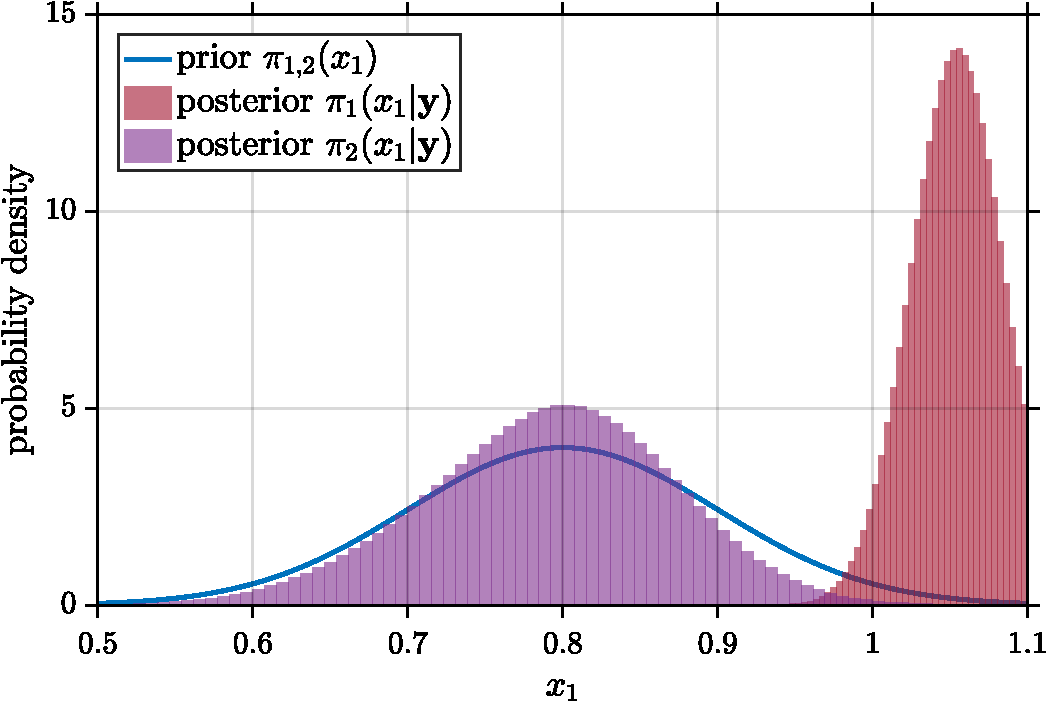
\includegraphics[height=\HYDROfigHeight]{fig_Hydro_Post12_x1}
    \caption{Model parameter \(x_1\).}
    \label{fig:Hydro:Post:x1}
  \end{subfigure}\hfill%
  \begin{subfigure}[b]{\HYDROsubWidth}
    \centering
    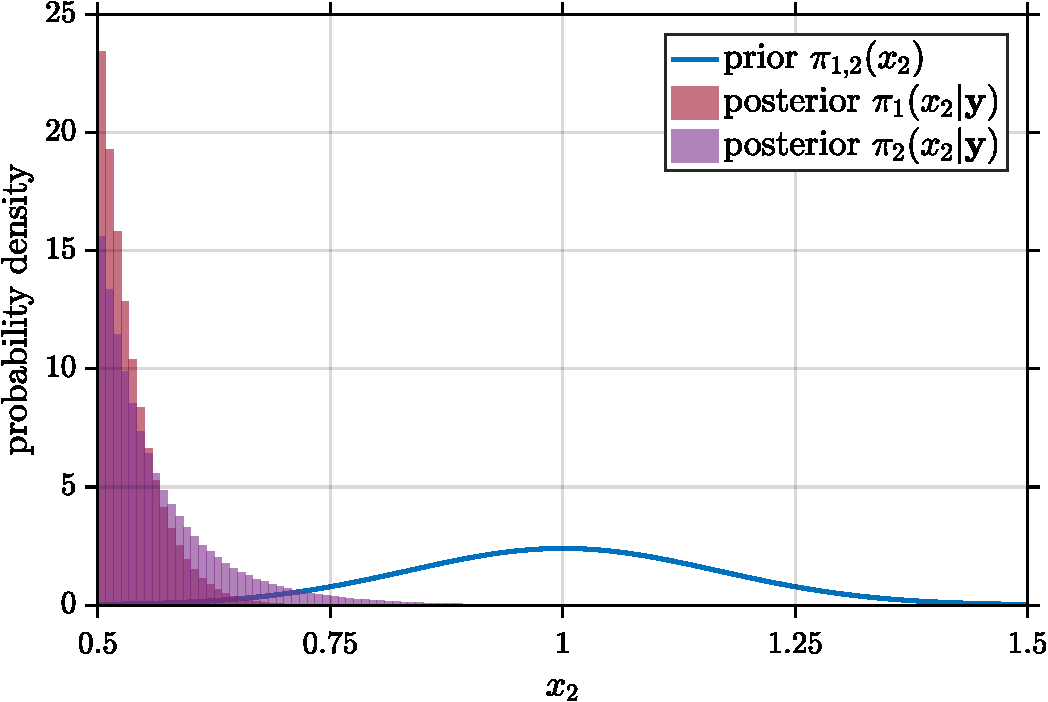
\includegraphics[height=\HYDROfigHeight]{fig_Hydro_Post12_x2}
    \caption{Model parameter \(x_2\).}
    \label{fig:Hydro:Post:x2}
  \end{subfigure}\\[1.4ex]%
  \begin{subfigure}[b]{\HYDROsubWidth}
    \centering
    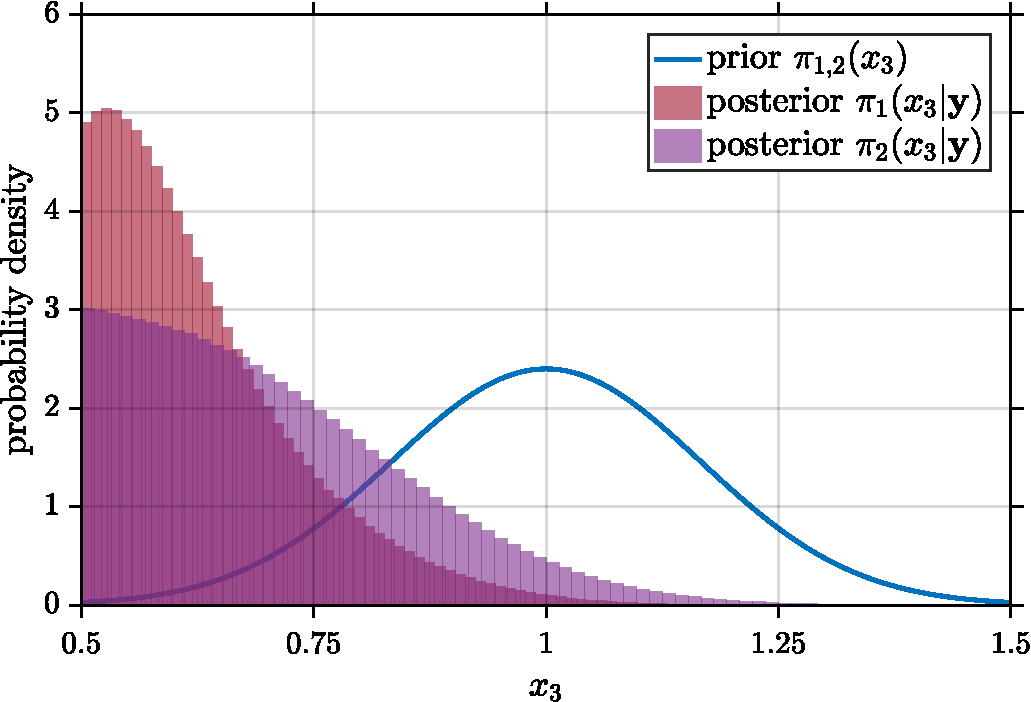
\includegraphics[height=\HYDROfigHeight]{fig_Hydro_Post12_x3}
    \caption{Model parameter \(x_3\).}
    \label{fig:Hydro:Post:x3}
  \end{subfigure}\hfill%
  \begin{subfigure}[b]{\HYDROsubWidth}
    \centering
    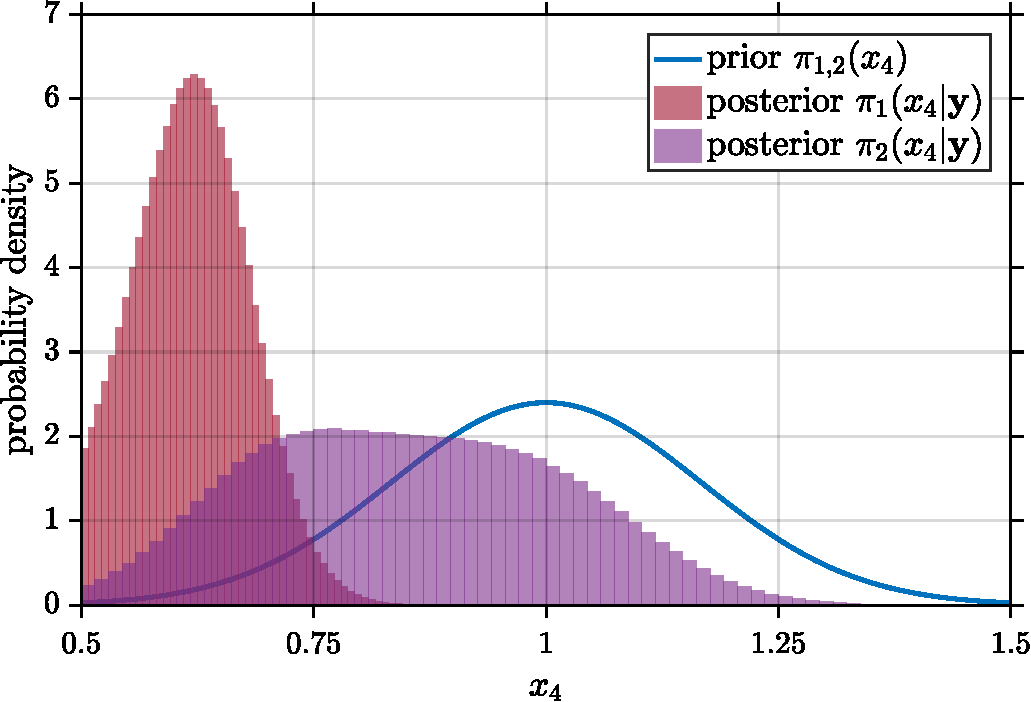
\includegraphics[height=\HYDROfigHeight]{fig_Hydro_Post12_x4}
    \caption{Model parameter \(x_4\).}
    \label{fig:Hydro:Post:x4}
  \end{subfigure}\\[1.4ex]%
  \begin{subfigure}[b]{\HYDROsubWidth}
    \centering
    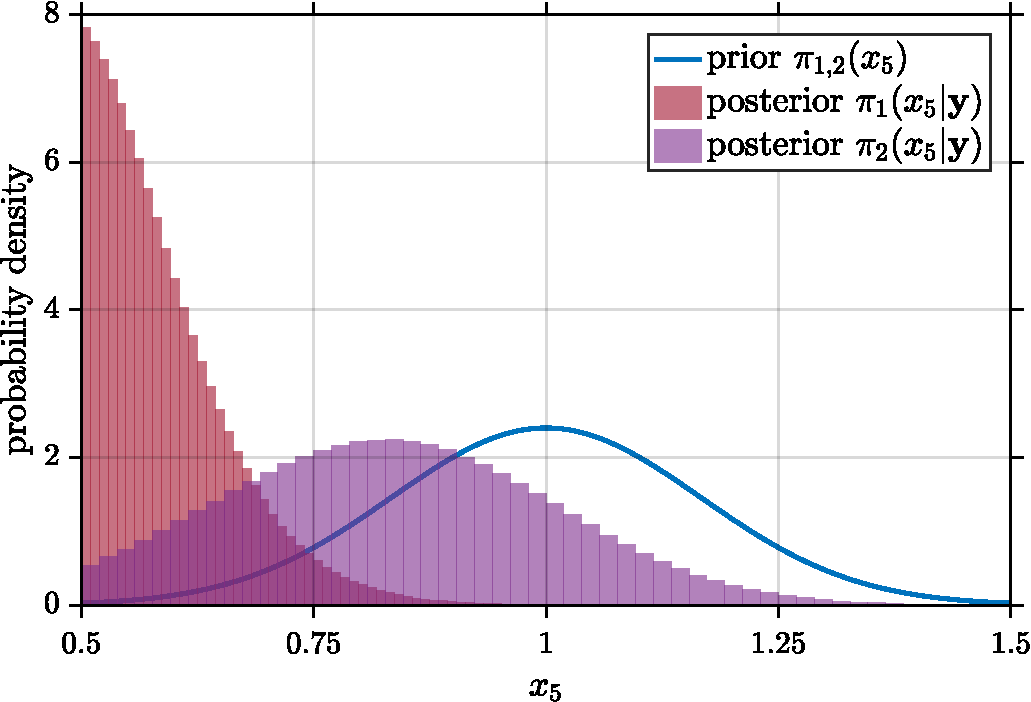
\includegraphics[height=\HYDROfigHeight]{fig_Hydro_Post12_x5}
    \caption{Model parameter \(x_5\).}
    \label{fig:Hydro:Post:x5}
  \end{subfigure}\hfill%
  \begin{subfigure}[b]{\HYDROsubWidth}
    \centering
    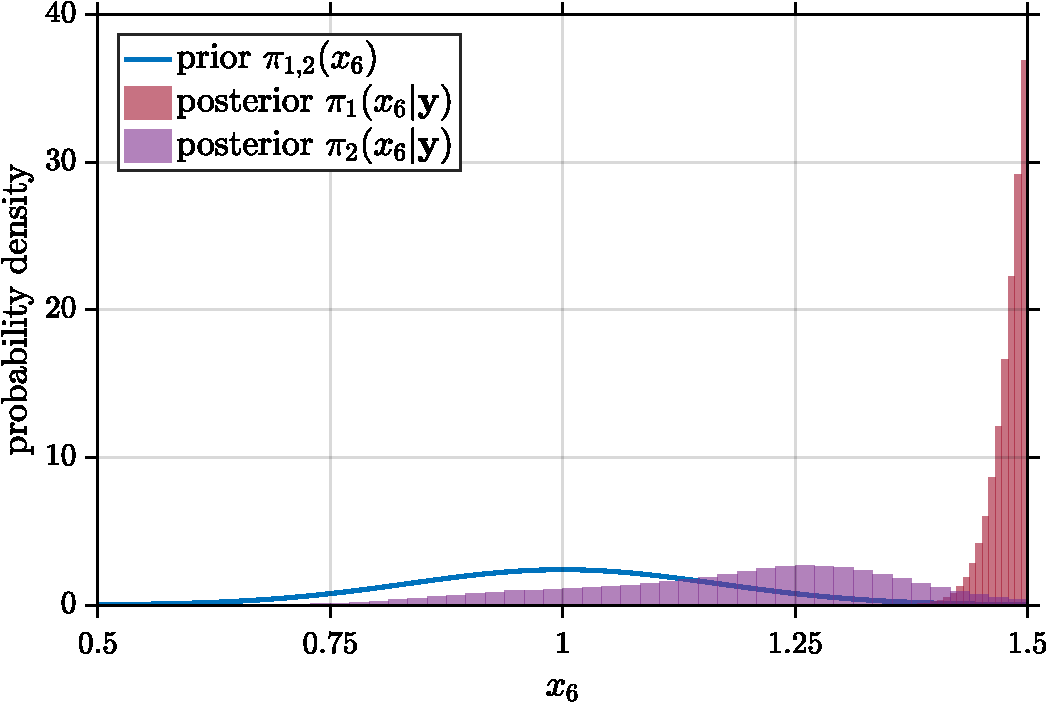
\includegraphics[height=\HYDROfigHeight]{fig_Hydro_Post12_x6}
    \caption{Model parameter \(x_6\).}
    \label{fig:Hydro:Post:x6}
  \end{subfigure}\\[1.4ex]%
  \begin{subfigure}[b]{\HYDROsubWidth}
    \centering
    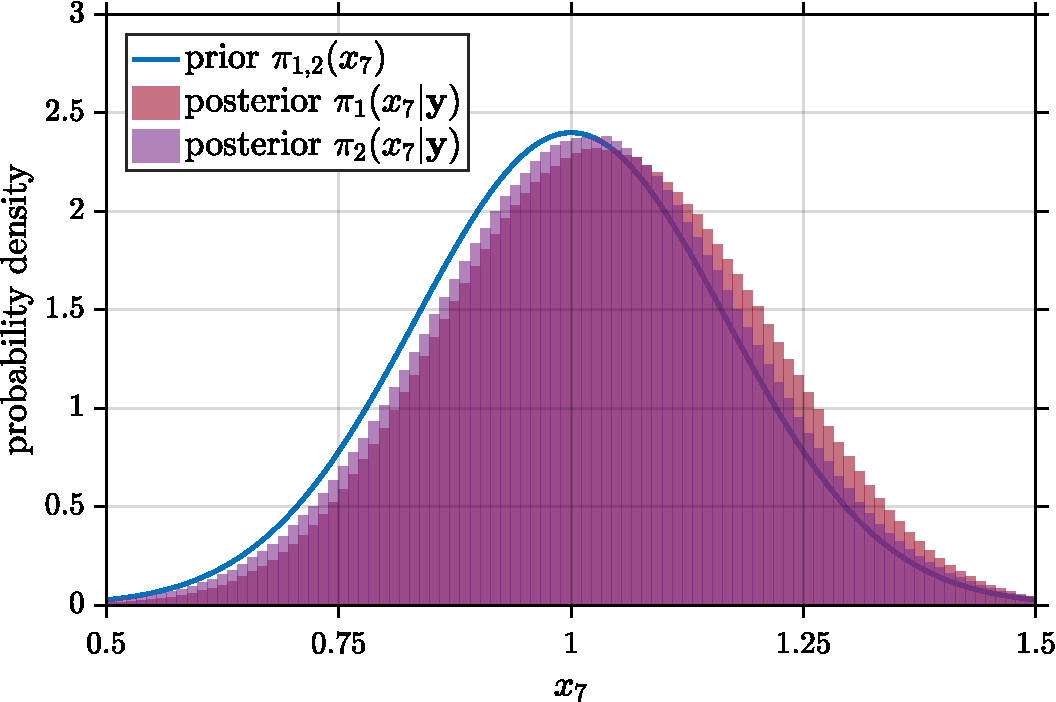
\includegraphics[height=\HYDROfigHeight]{fig_Hydro_Post12_x7}
    \caption{Model parameter \(x_7\).}
    \label{fig:Hydro:Post:x7}
  \end{subfigure}\hfill%
  \begin{subfigure}[b]{\HYDROsubWidth}
    \centering
    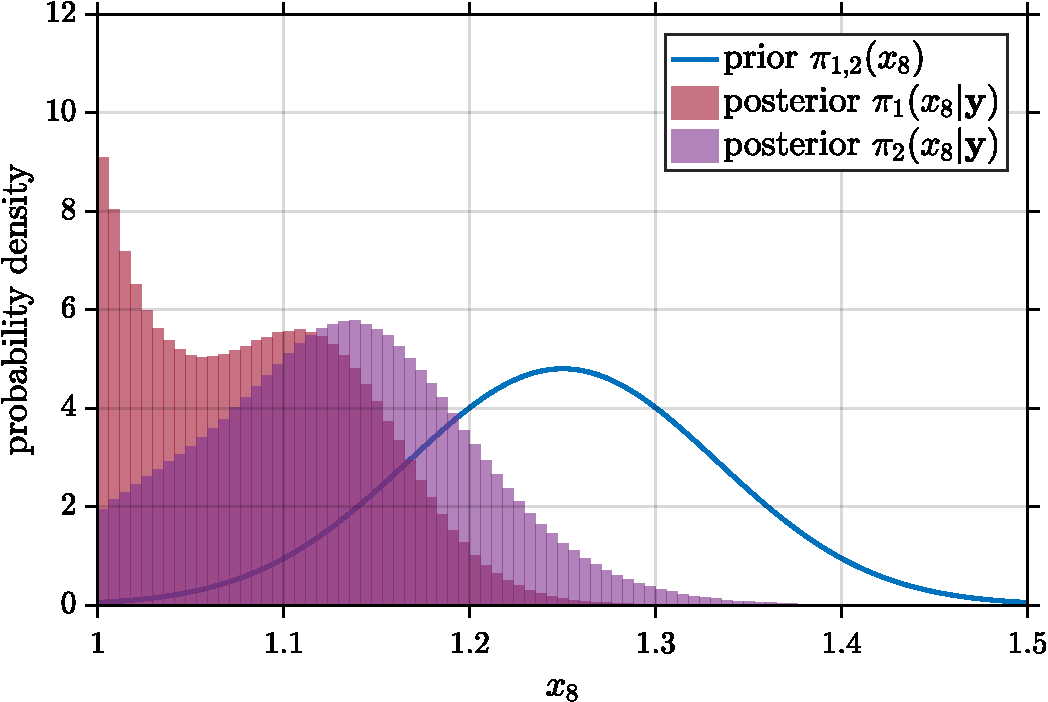
\includegraphics[height=\HYDROfigHeight]{fig_Hydro_Post12_x8}
    \caption{Model parameter \(x_8\).}
    \label{fig:Hydro:Post:x8}
  \end{subfigure}%
  \caption[Posterior marginals for the hydrological model]{Posterior marginals for the hydrological model.}
  \label{fig:Hydro:Post:Parameters}
\end{figure}
\par % ERROR MODEL
The posterior marginals of the parameters describing the random error model are shown in \cref{fig:Hydro:Post:ErrorModel}.
% STANDARD DEVIATION
As it can be seen from \cref{fig:Hydro:Post:Sigma}, the marginal \(\pi_1(\sigma \cond \bm{y})\)
suggests a higher value of the standard deviation \(\sigma\) than the marginal \(\pi_2(\sigma \cond \bm{y})\).
The reason is that according to the first model all errors are attributed to independent noise only.
% CORRELATION LENGTH
In the second model, those errors are also captured by the error correlation and model discrepancy.
The marginal \(\pi_2(\tau \cond \bm{y})\) of the correlation length \(\tau\) is plotted in \cref{fig:Hydro:Post:Tau}.
It concentrates around a surprisingly low value.
We speculate that the introduction and estimation of the discrepancy term effectively decorrelates the remaining sources of random error, which would explain this observation.
% DISCREPANCY COEFFICIENTS
In \cref{fig:Hydro:Post:DiscrepancyModel} all marginals \(\pi_2(b_i \cond \bm{y})\) of the coefficients \(b_i\) with \(i=0,\ldots,5\) are shown.
Their actual units are discarded for the sake of simplicity.
It is interesting to note that the parameters \(\bm{b}\) of the discrepancy function are estimated quite clearly.
Especially the constant and the linear term with their coefficients \(b_0\) and \(b_1\) have pronounced posterior shapes.
% FIGURES: POSTERIOR MARGINALS OF RANDOM ERROR MODEL
\begin{figure}[htbp]
  \centering
  \begin{subfigure}[b]{\HYDROsubWidth}
    \centering
    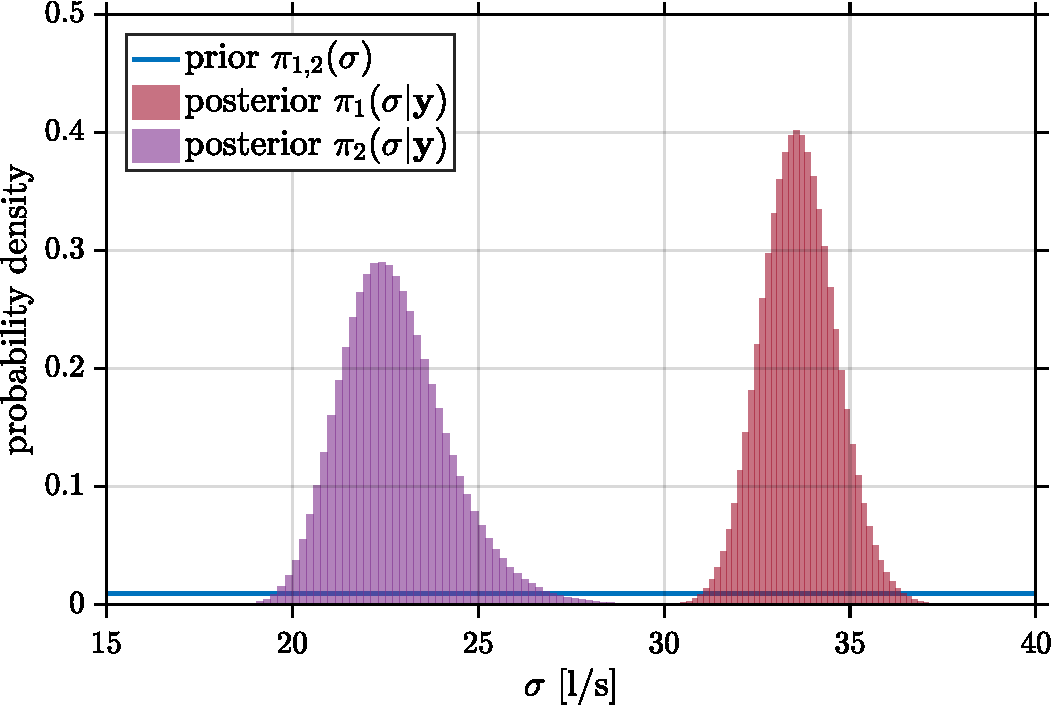
\includegraphics[height=\HYDROfigHeight]{fig_Hydro_Post12_Sigma}
    \caption{Noise level \(\sigma\).}
    \label{fig:Hydro:Post:Sigma}
  \end{subfigure}\hfill%
  \begin{subfigure}[b]{\HYDROsubWidth}
    \centering
    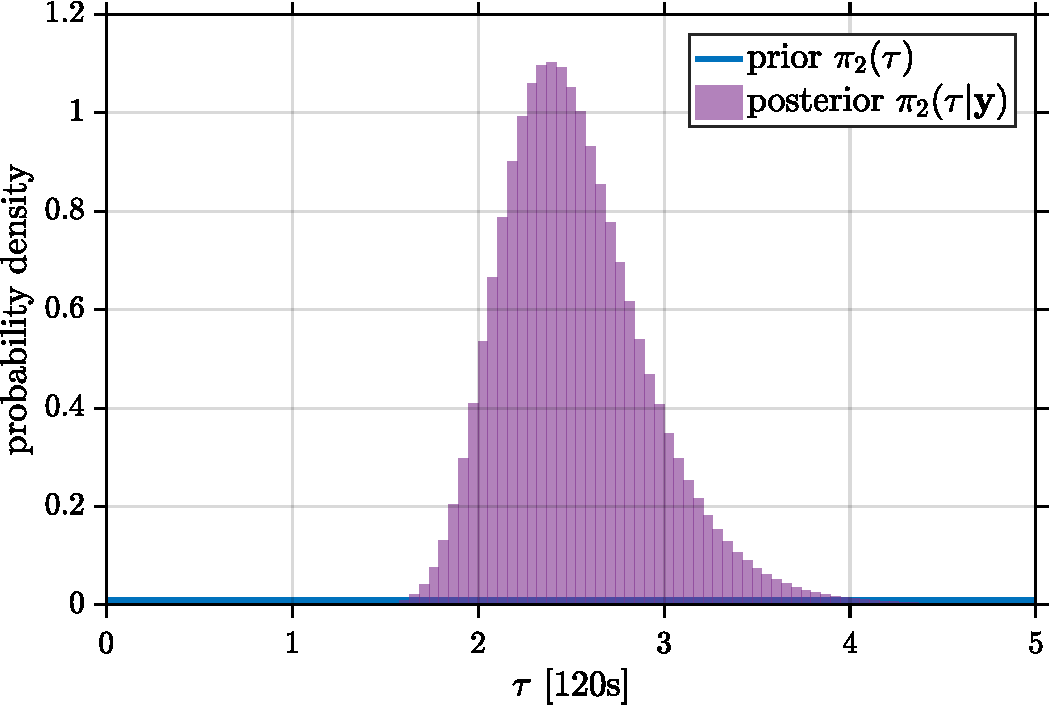
\includegraphics[height=\HYDROfigHeight]{fig_Hydro_Post2_Tau}
    \caption{Correlation length \(\tau\).}
    \label{fig:Hydro:Post:Tau}
  \end{subfigure}\\[1.5ex]%
  \begin{subfigure}[b]{\HYDROsubWidth}
    \centering
    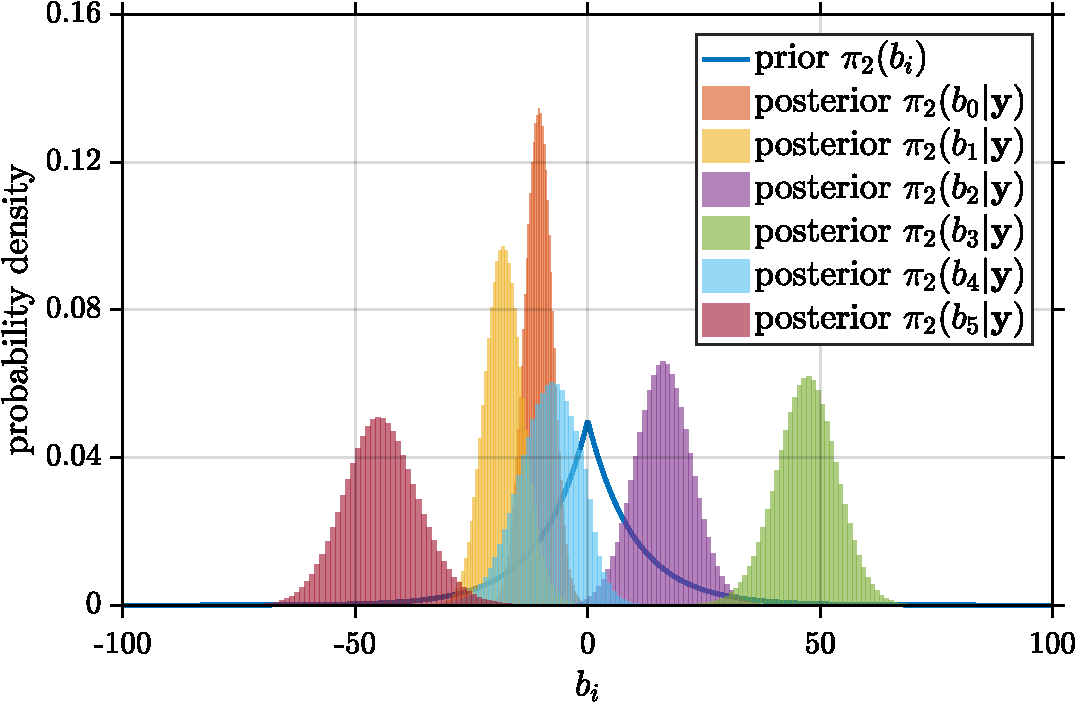
\includegraphics[height=\HYDROfigHeight]{fig_Hydro_Post2_b}
    \caption{Discrepancy coefficients \(b_i\).}
    \label{fig:Hydro:Post:DiscrepancyModel}
  \end{subfigure}%
  \caption[Posterior marginals for the error model]{Posterior marginals for the error model.}
  \label{fig:Hydro:Post:ErrorModel}
\end{figure}
\par % POSTERIOR SUMMARIES
Some summaries of the posterior distributions \(\pi_1(\bm{x},\sigma \cond \bm{y})\) and \(\pi_2(\bm{x},\bm{b},\sigma,\tau \cond \bm{y})\) are compiled in \cref{tab:Hydro:Post:Summaries}.
These are point estimates of the unknown parameters, e.g.\ the posterior mean vectors \((\hat{\bm{x}},\hat{\sigma}) = \mathds{E}[\bm{x},\sigma \cond \bm{y}]\)
and \((\hat{\bm{x}},\hat{\bm{b}},\hat{\sigma},\hat{\tau}) = \mathds{E}[\bm{x},\bm{b},\sigma,\tau \cond \bm{y}]\).
Quantities whose dimension does not equal one are expressed in comparison to the units that were previously adopted.
Posteriors that peak at the prior bounds are not summarized well by their mean values only.
Therefore the modes \((\hat{\bm{x}},\hat{\sigma})_{\mathrm{MAP}} = \operatorname{arg\,max}_{\bm{x},\sigma} \pi_1(\bm{x},\sigma \cond \bm{y})\) and
\((\hat{\bm{x}},\hat{\bm{b}},\hat{\sigma},\hat{\tau})_{\mathrm{MAP}} = \operatorname{arg\,max}_{\bm{x},\bm{b},\sigma,\tau} \pi_2(\bm{x},\bm{b},\sigma,\tau \cond \bm{y})\)
of the joint posterior densities are shown, too.
They have been obtained through maximizing the logarithms of the unnormalized posterior densities, i.e.\ the log--likelihood function plus the log--prior density.
Note that the individual components of the joint posterior density mode do not have to coincide with the maxima of the marginal densities.
% TABLE: POSTERIOR SUMMARIES
\begin{table}[htbp]
  \caption[Posterior summaries]{Posterior summaries.}
  \label{tab:Hydro:Post:Summaries}
  \centering
  \resizebox{\linewidth}{!}{
  \begin{tabular}{llcccccccccccccccc}
    \toprule
    & & \(\hat{x}_1\) & \(\hat{x}_2\) & \(\hat{x}_3\) & \(\hat{x}_4\) & \(\hat{x}_5\) & \(\hat{x}_6\) & \(\hat{x}_7\) & \(\hat{x}_8\)
    & \(\hat{\sigma}\) & \(\hat{\tau}\) & \(\hat{b}_0\) & \(\hat{b}_1\) & \(\hat{b}_2\) & \(\hat{b}_3\) & \(\hat{b}_4\) & \(\hat{b}_5\) \\
    \midrule
    \multirow{2}{*}{\(\pi_1(\cdot \cond \bm{y})\)}
    & Mean
    & \(1.05\) & \(0.54\) & \(0.63\) & \(0.62\) & \(0.59\) & \(1.48\) & \(1.04\) & \(1.09\) & \(33.63\)
    & - & - & - & - & - & - & - \\
    & Mode
    & \(1.06\) & \(0.50\) & \(0.55\) & \(0.62\) & \(0.50\) & \(1.49\) & \(0.99\) & \(1.00\) & \(33.04\)
    & - & - & - & - & - & - & - \\
    \multirow{2}{*}{\(\pi_2(\cdot \cond \bm{y})\)}
    & Mean
    & \(0.79\) & \(0.56\) & \(0.70\) & \(0.85\) & \(0.84\) & \(1.18\) & \(1.02\) & \(1.13\) & \(22.78\) & \(2.53\) & \(-10.63\) & \(-17.97\) & \(16.33\) & \(47.05\) & \(-8.38\) & \(-44.31\) \\
    & Mode
    & \(0.71\) & \(0.50\) & \(0.50\) & \(0.71\) & \(0.59\) & \(0.91\) & \(1.01\) & \(1.03\) & \(19.95\) & \(1.80\) & \(-13.33\) & \(-20.25\) & \(19.39\) & \(46.70\) & \(-10.25\) & \(-42.72\) \\
    \bottomrule
  \end{tabular}
  }
\end{table}
\par % PRIOR/POSTERIOR PREDICTIONS
After having explored the posterior distribution, one can check the obtained results for consistency by comparing an ensemble of prior and posterior predictions with the data.
We start by comparing the posterior \(\pi_1(\bm{x},\sigma \cond \bm{y})\) of the first model with the correspondent prior \(\pi_1(\bm{x},\sigma)\) in this regard.
See \cref{fig:Hydro:PCE} for that purpose.
In \cref{fig:Hydro:PCE:Prior} the forecasts of the outflow are shown for one hundred input values that were randomly sampled from the prior.
Likewise \cref{fig:Hydro:PCE:Posterior} shows the predictions for the same number of posterior samples that were obtained from the MCMC chains by an appropriate thinning.
Moreover, the time trajectory for the posterior mode is highlighted.
The measurement uncertainty is not accounted for in those figures.
As it can be seen, the prediction ensemble for the prior contains more uncertainty than for the posterior.
\par % SYSTEMATIC DISCREPANY
The adjustment of the model parameters associated with the Bayesian update does not significantly reduce
the systematic discrepancy between the simulated and the measured outflows from the drainage basin.
The underlying reason is that varying the input parameters of the hydrological simulator and the level of independent noise
does not allow for establishing full consistency between the simulations and the observations, especially in the second half of the covered time interval.
This was already clear after the discussion of \cref{fig:Hydro:Data:Outflow} and actually led to the inclusion of a correlation and discrepancy term in the second model.
% FIGURES: PRIOR/POSTERIOR PCE PREDICTIONS
\begin{figure}[htbp]
  \centering
  \begin{subfigure}[b]{\HYDROsubWidth}
    \centering
    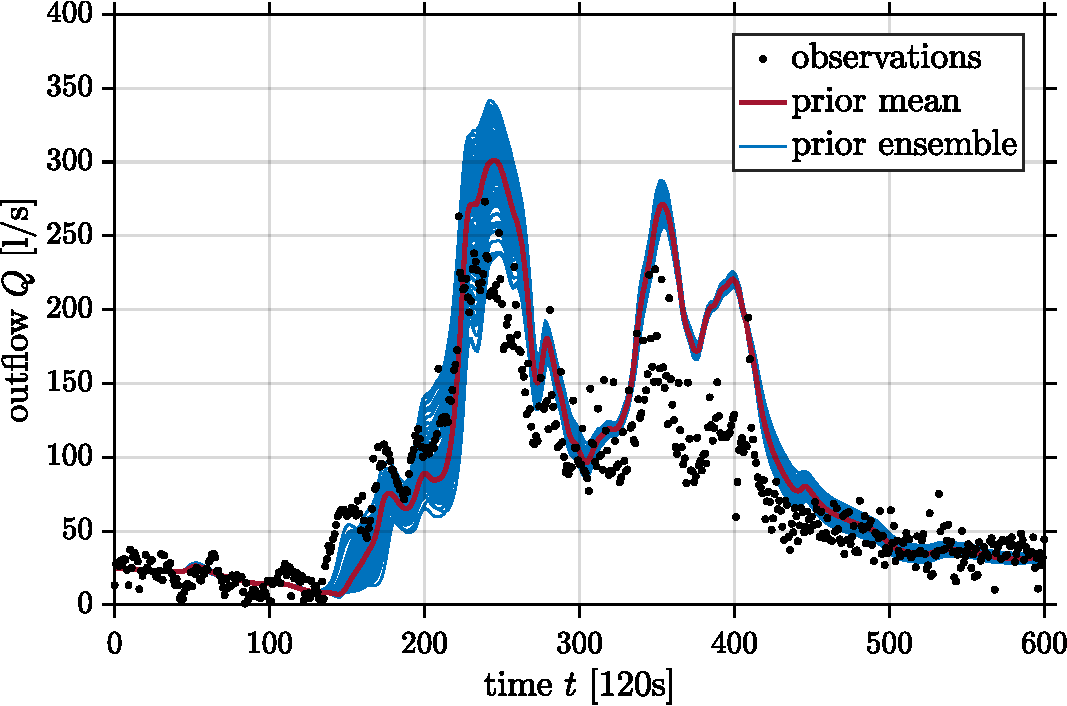
\includegraphics[height=\HYDROfigHeight]{fig_Hydro_PCE_Prior}
    \caption{Prior predictions.}
    \label{fig:Hydro:PCE:Prior}
  \end{subfigure}\hfill%
  \begin{subfigure}[b]{\HYDROsubWidth}
    \centering
    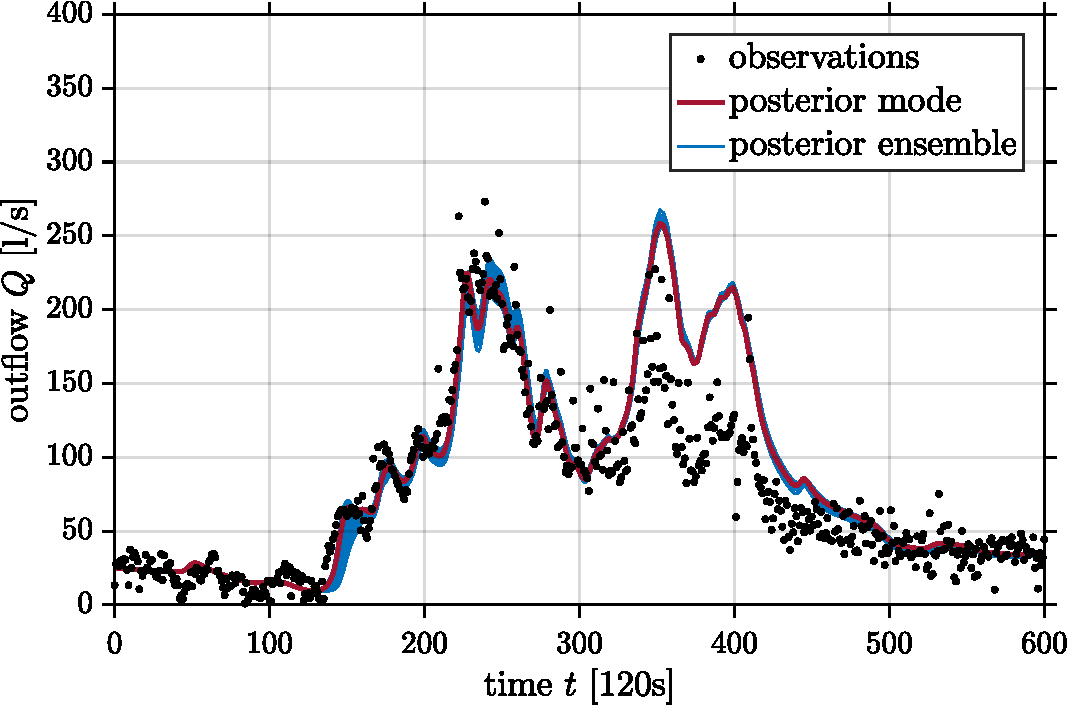
\includegraphics[height=\HYDROfigHeight]{fig_Hydro_PCE_Post}
    \caption{Posterior predictions.}
    \label{fig:Hydro:PCE:Posterior}
  \end{subfigure}%
  \caption[Stochastic model predictions]{Stochastic model predictions.}
  \label{fig:Hydro:PCE}
\end{figure}
\par % CORRECTED PREDICTIONS
We now investigate how well the posterior mode of \(\pi_2(\bm{x},\bm{b},\sigma,\tau \cond \bm{y})\) aligns with the data.
The mode estimate of the discrepancy function \(\hat{\delta}(t) = \delta(\hat{\bm{b}},t)\) is plotted in \cref{fig:Hydro:MAP:Discrepancy}.
It indicates a trend that the model underpredicts the actual rainfall in roughly the interval \(t / \unit[120]{s} \in [100,250]\) and overpredicts in \(t / \unit[120]{s} \in [250,500]\).
These mis-predictions occur more or less for the period \(t / \unit[120]{s} \in [100,450]\) of the precipitation event that was shown in \cref{fig:Hydro:Data:Rainfall}.
At the boundaries, say for \(t / \unit[120]{s} \in [0,100]\) and \(t / \unit[120]{s} \in [500,600]\), the discrepancy vanishes as far as the low-degree polynomial representation admits.
The accordingly corrected predictions \(\hat{\mathcal{M}}_p(\hat{\bm{x}}) + \hat{\bm{\delta}}\) are depicted in  \cref{fig:Hydro:MAP:Predictions}.
They align with the data reasonably well.
One, two and three \(\hat{\sigma}\) prediction intervals are added so as to visualize the posterior mode prediction uncertainty.
% NEGATIVE OUTFLOWS
Due to the additive and symmetric error model, the intervals extend to negative outflow values.
Since these values are physically nonsensical, they shall be ignored.
% FIGURES: MAP CORRECTIONS
\begin{figure}[htbp]
  \begin{minipage}[b]{\HYDROsubWidth}
    \centering
    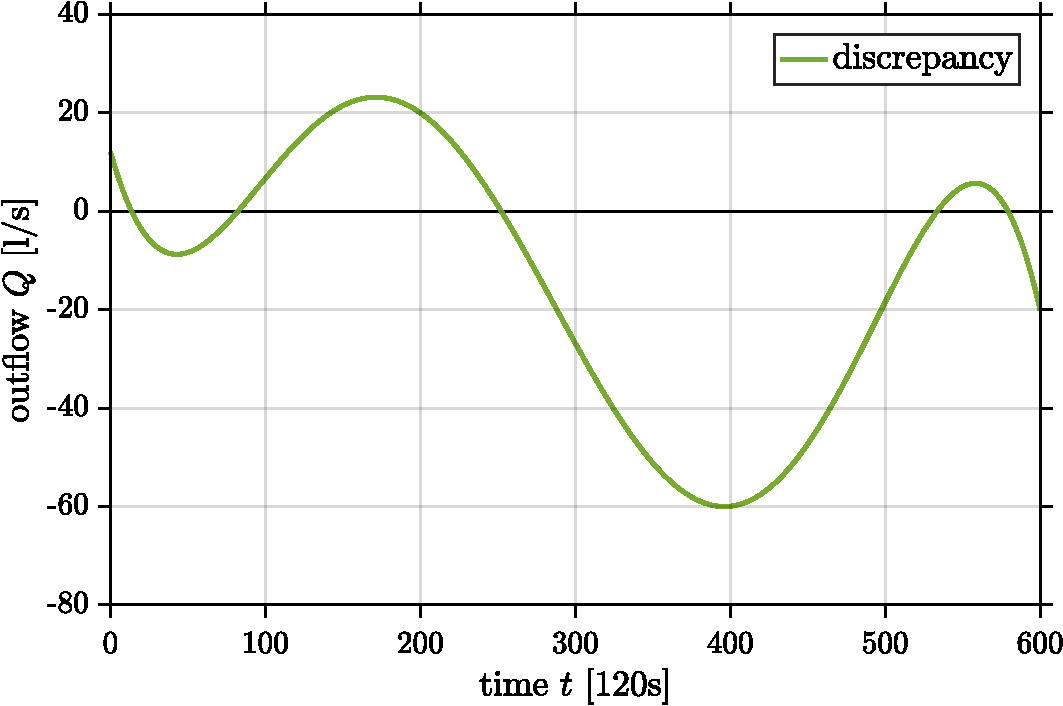
\includegraphics[height=\HYDROfigHeight]{fig_Hydro_MAP_Discrepancy}
    \caption[Model discrepancy]{Model discrepancy.}
    \label{fig:Hydro:MAP:Discrepancy}
  \end{minipage}%
  \hfill%
  \begin{minipage}[b]{\HYDROsubWidth}
    \centering
    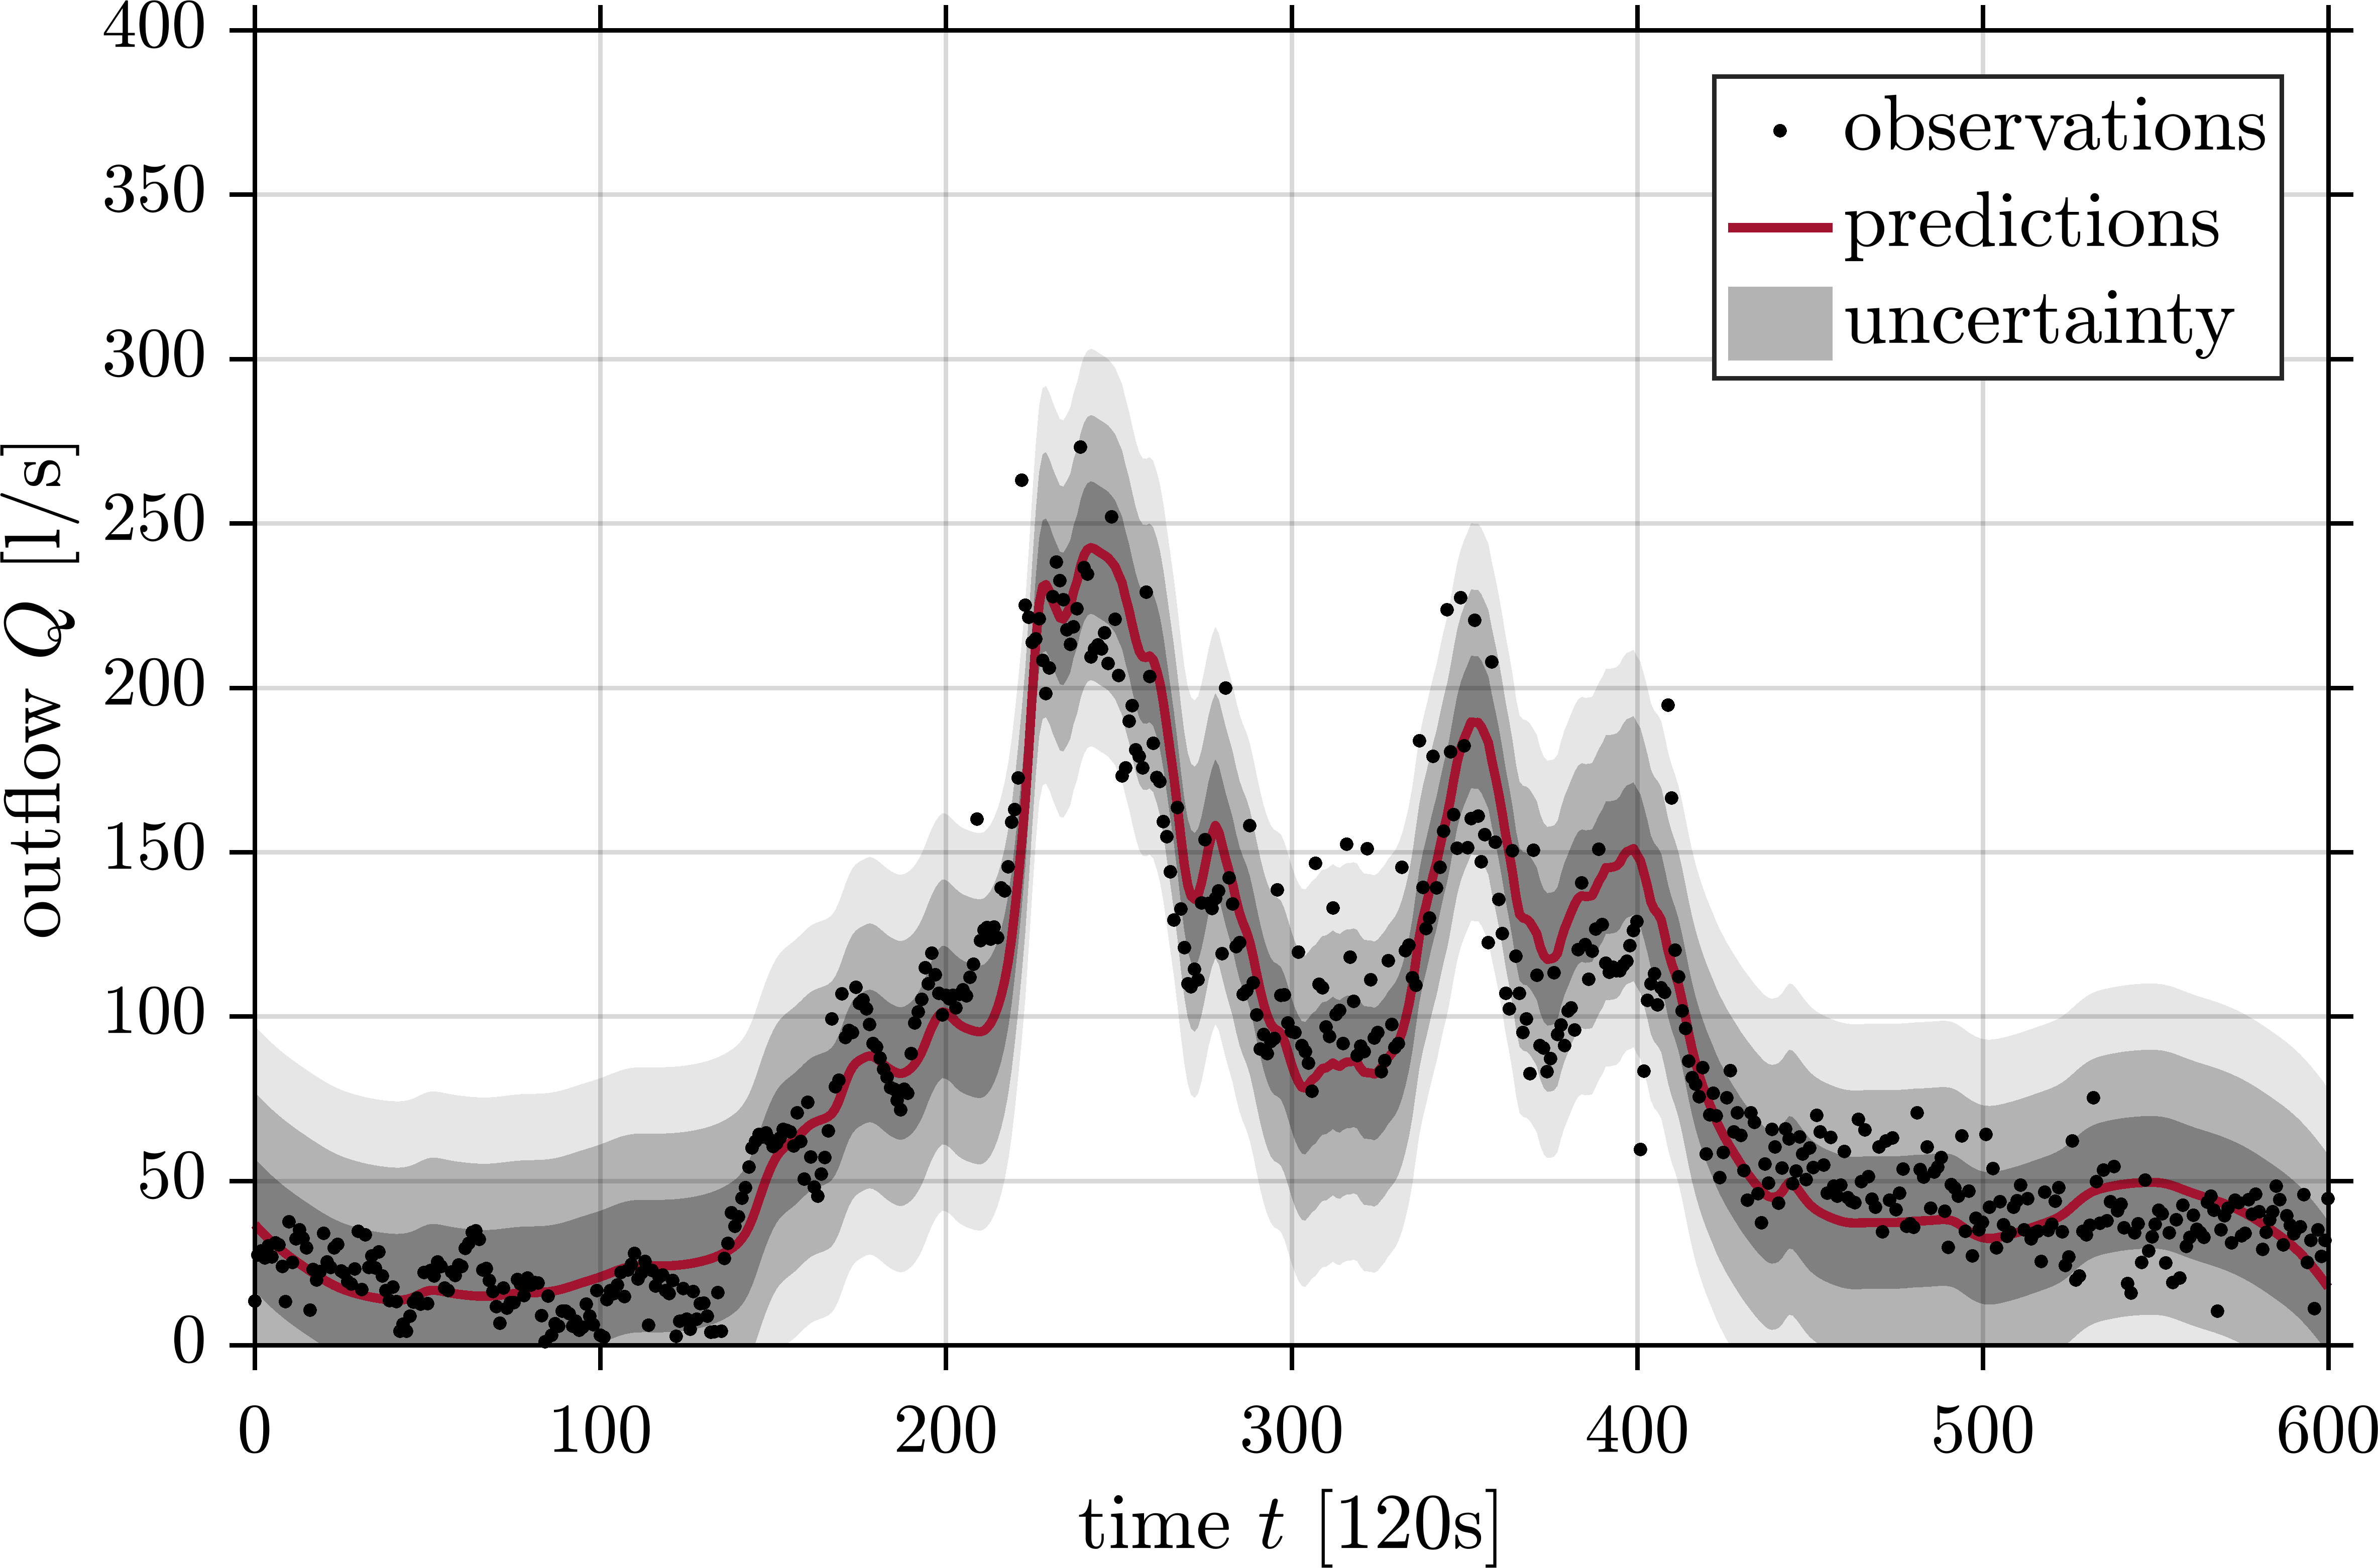
\includegraphics[height=\HYDROfigHeight]{fig_Hydro_MAP_Predictions}
    \caption[Corrected predictions]{Corrected predictions.}
    \label{fig:Hydro:MAP:Predictions}
  \end{minipage}%
\end{figure}